
\documentclass[ExampleMasters.tex]{subfiles}
\begin{document}

	\chapter{APPENDIX A}
	{\Large Genetic Algorithm Implementation and testing in C++}

	\section{Elements of a standard Genetic Algorithm}
		The genetic algorithm draws inspiration from evolutionary processes seen in nature. Several randomly generated individuals are allowed to \textit{mate} and share genetic data and efficient \textit{stronger} individuals tend to be selected for such information transfers more often than \textit{weaker} individuals with characteristics that drive the objective function lower. Selected individuals mate and exchange genetic information producing offspring with strong genetic makeup and characteristics that replace the existing population. Occasional probabilistic genetic mutations help in discovering potentially \textit{strong} genome sequences that may accelerate the evolution of the species. While variations in any or all of these processes alter the efficacy of the algorithm, the prevalence of \textit{stronger} individuals over \textit{weaker} ones drives the evolution over several pre-defined number of generations.\\

		\subsection{Objective Function}
			The purpose of the optimisation technique is to identify the global maximum or minimum of a desired objective function that is defined in one or several variables / parameters. Such a function is mathematically constructed and a range within which the function optimum is desired is defined. For example, the two-variable benchmark Goldstein-Price function is defined as:
			\begin{multline}
				f(x,y)=(1+(x+y+1)^2(19-14x+3x^2-14y+6xy+3y^2))\\
					(30+(2x-3y)^2(18-32x+12x^2+48y-36xy+27y^2))
			\end{multline}

			whose global minima lies at $x=0$ and $y=-1$ and $f(0,-1)=-3$. In this research, the objective function to be maximised is the combination productivity as described in Chapter 2.\\

		\subsection{Individual representation and creation}
			The variables of the above defined objective function may be represented as a genetic sequence in a manner that allows a variety of data points where the function is defined to be created. Each set of data points $(x,y)$ may be called an \textit{individual}. Such individuals are often \textit{encoded} in binary or real-number formats. For example, an individual \textit{chromosome} containing 10 bits, 5 consecutive bits representing each variable $x$ and $y$ may look like:

			$$ 0     0     1     0     0     1     1     1     0     1$$

			The bits representing the encoded individual are the genetic material that is exchanged upon mating. A pre-defined number of such individuals constituting a \textit{population} form the breeding ground for the evolutionary exercise leading to the optimal solution. The individual structure and encoding scheme may, of course, vary to suit the problem at hand. The population of individuals is created stochastically using a pseudo-random number generator engine that generate integers based on a uniform distribution.\\

			\begin{figure}[H]
				\centering
				\includegraphics[width=0.6\linewidth]{figures/GeneticAlgorithm/GA1}
				\caption{Genetic Algorithm - Initialisation}
				\label{GA1}
			\end{figure}

		\subsection{Decoding, Evaluation and Selection}
			Created individuals are decoded based on pre-set rules and the function value represented by each individual in the population is evaluated. For example, the above shown individual may be decoded to $(x,y) = (-2.2258, 2.6129)$. The Goldstein Price function defined above is evaluated to a value of $0.1711$ at this data point and is thus assigned as the individual's \textit{fitness}. From this created population, 2 or more individuals are \textit{selected} probabilistically and either repetitively or uniquely. Selected individuals mate to produce \textit{offspring} that replace the \textit{parents} in the population. Tournament selection and Roulette-wheel selection are often employed as stochastic selection mechanisms where the \textit{fitter} individual is selected over the \textit{weaker} with a preset probability.\\

			\begin{figure}[H]
				\centering
				\includegraphics[width=0.6\linewidth]{figures/GeneticAlgorithm/GA2}
				\caption{Genetic Algorithm - Evaluation}
				\label{GA2}
			\end{figure}

			\begin{figure}[H]
				\centering
				\includegraphics[width=0.6\linewidth]{figures/GeneticAlgorithm/GA3}
				\caption{Genetic Algorithm - Selection}
				\label{GA3}
			\end{figure}

		\subsection{Crossover}
			Such selected individuals exchange different portions of their genetic makeup in a stochastic fashion based on a pre-defined crossover probability. For example, individuals such as the ones shown above may be split at a random bit location beyond which all bits are exchanged with the other selected individual or individuals.\\ 

			\begin{figure}[H]
				\centering
				\includegraphics[width=0.6\linewidth]{figures/GeneticAlgorithm/GA4}
				\caption{Genetic Algorithm - Crossover}
				\label{GA4}
			\end{figure}

		\subsection{Mutation}
			Mimicking natural mutation processes that create varieties in genetic makeup leading to new features, random bits may, with a mutation probability, be mutated to another value. This may occassionally produce very fit individuals that can accelerate the evolution of the generation.\\

			\begin{figure}[H]
				\centering
				\includegraphics[width=0.7\linewidth]{figures/GeneticAlgorithm/GA5}
				\caption{Genetic Algorithm - Mutation}
				\label{GA5}
			\end{figure}

		\subsection{Elitism}
			The fittest individual in each generation may be preserved at the end of the generation so as to ensure that the information producing the best function values in that generation are not lost leading to oscillating best individual fitnesses in successive generations.\\

		These processes repeat for a number of decided generations until all individuals converge to the \textit{Vitruvian} individual representing the global optima of the objective function chosen to be optimised.\\

		\begin{figure}[H]
			\centering
			\includegraphics[width=0.7\linewidth]{figures/GeneticAlgorithm/GA7}
			\caption{Genetic Algorithm - Optimal solution}
			\label{GA7}
		\end{figure}

		% \begin{figure}[ht!]
		% 	\centering
		% 	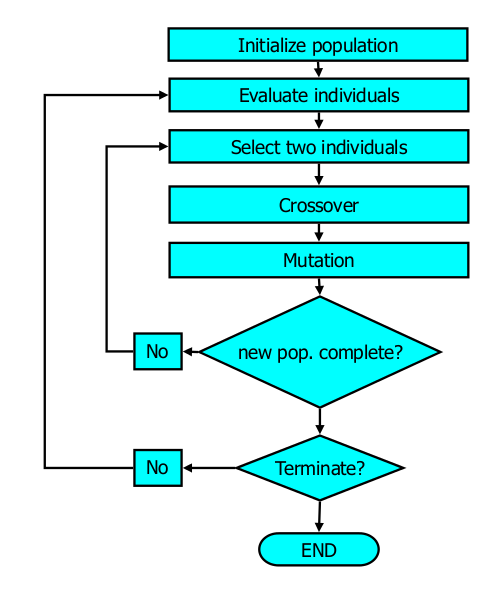
\includegraphics[width=0.4\linewidth]{figures/GeneticAlgorithm/GAFlowchart.png}
		% 	\caption{Genetic Algorithm Description Flowchart \cite{Wahde}}
		% 	\label{GAFlowchart}
		% \end{figure}


	\section{Implementation and validation}
		The standard genetic algorithm constructed using selection, crossover and mutation over successive generations is implemented using the C++ programming language. The choice of C++ over the standard engineering programming tool, \verb!MATLAB!, is justified by the need for quick computations and reduced running time in light of the large number of computations that are involved in the solution of the target optimisation problem. \\

		While the algorithm has earlier been implemented and tested in \verb!MATLAB!, the object oriented structure that C++ necessitates lends a more complete and integrated solution structure when combined with the propulsion optimisation problem at hand. To begin with, a simple genetic algorithm was constructed in C++ in a manner so as to insulate the algorithm engine from the function to be optimised. This renders a generic solver that can later be adapted to specific optimisation problems. The so-constructed algorithm was first tested using three standard benchmark functions that are used to evaluate the performance of optimisation schemes in the literature:
		\begin{itemize}
			\item Goldstein Price Function
			\item Beale's Function
			\item Booth's function
		\end{itemize}

		The minimae of the three functions listed above were verified using the algorithm and the solution code was thus tested to be reliable and consistent across repeated refreshed runs of the algorithm.\\

	\section{Algorithm performance for benchmark functions}

		Standard two-dimensional functions are used to benchmark optimisation schemes and validate the optimas indicated by the scheme at hand. A similar mode of evaluation is employed here and the convergence of the population to the optima in each case tracked. In addition, the fitness of the fittest individual in each generation and the convergence of the best fitness with increasing generation number is observed. Below are plots of the population and fitness over 500 generations, each consisting of 30 individuals.\\ 

		\subsection{Goldstein Price Function}

			The Goldstein Price function in 2 variables is given by:
			%\begin{equation}
			\begin{multline}
				f(x,y)=(1+(x+y+1)^2(19-14x+3x^2-14y+6xy+3y^2))\\
					(30+(2x-3y)^2(18-32x+12x^2+48y-36xy+27y^2))
			\end{multline}
			%\end{equation}

			The minima of the Goldstein Price function lies at (x,y)=(0,-1) and the function value at the minima is -3. This is verified by the algorithm outputs.

			\begin{figure}[hb!]
				\centering
				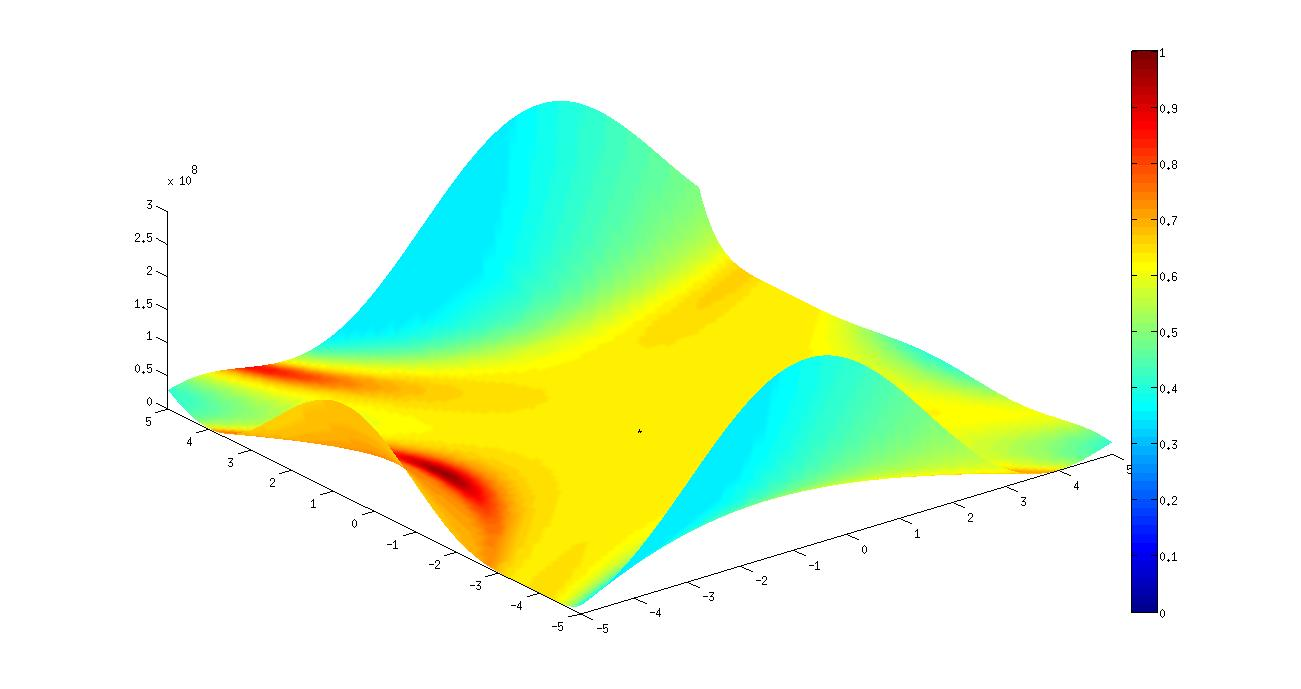
\includegraphics[width=\textwidth]{figures/GeneticAlgorithm/GPR.jpg}
				\caption{Goldstein Price Function}
				\label{GPR}
			\end{figure}

			\begin{figure}[hb!]
				\centering
				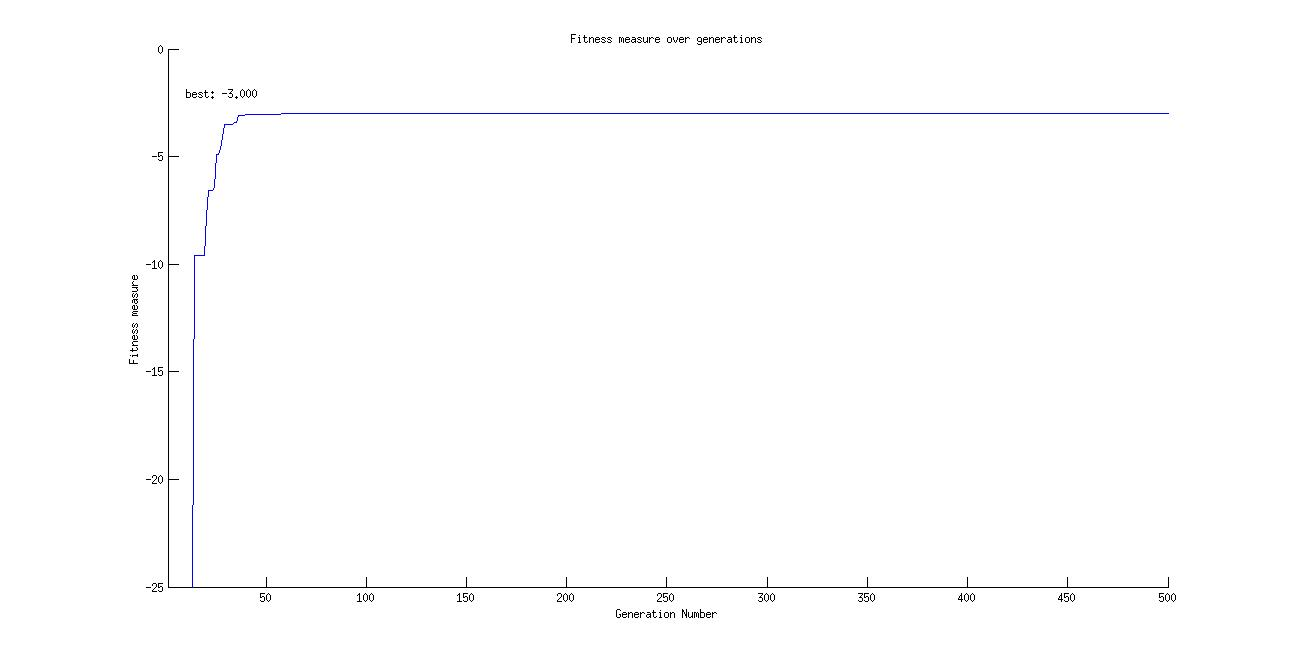
\includegraphics[width=\textwidth]{figures/GeneticAlgorithm/GPR_fitness_vs_generation.jpg}
				\caption{Progress of population best fitness over generations, Goldstein Price Function}
				\label{GPRF}
			\end{figure}

			\begin{figure}[ht!]
				\begin{subfigure}[b]{0.5\textwidth}
					\centering
					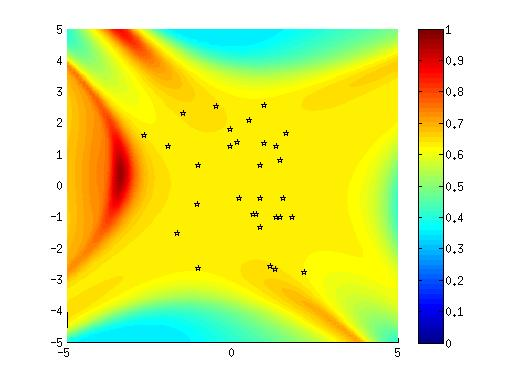
\includegraphics[width=\textwidth]{figures/GeneticAlgorithm/GPR1.jpg}
					\caption{\centerline{First generation\\ Goldstein Price Function}}
					\label{GPR1}
				\end{subfigure}
				\quad
				\begin{subfigure}[b]{0.5\textwidth}
					\centering
					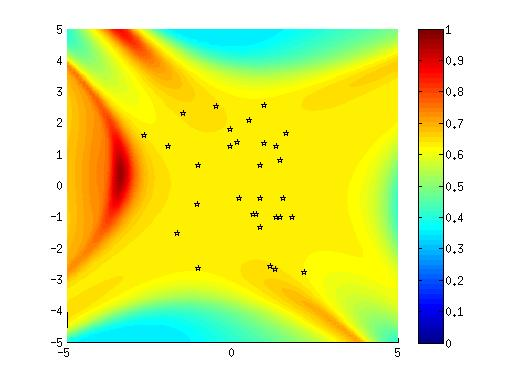
\includegraphics[width=\textwidth]{figures/GeneticAlgorithm/GPR2.jpg}
					\caption{\centerline{Third generation\\ Goldstein Price Function}}
					\label{GPR2}
				\end{subfigure}

				\begin{subfigure}[b]{0.5\textwidth}
					\centering
					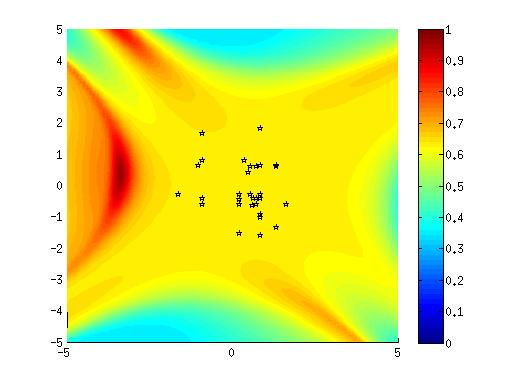
\includegraphics[width=\textwidth]{figures/GeneticAlgorithm/GPR4.jpg}
					\caption{\centerline{Fifth generation\\ Goldstein Price Function}}
					\label{GPR3}
				\end{subfigure}
				\quad
				\begin{subfigure}[b]{0.5\textwidth}
					\centering
					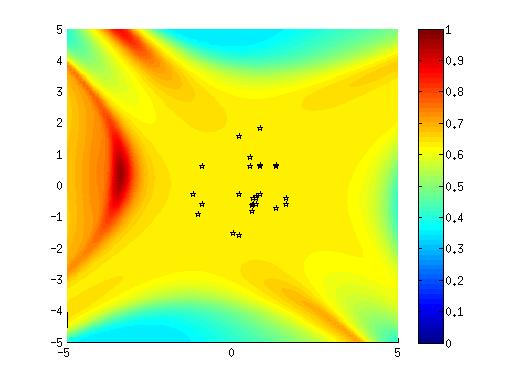
\includegraphics[width=\textwidth]{figures/GeneticAlgorithm/GPR5.jpg}
					\caption{\centerline{Ninth generation\\ Goldstein Price Function}}
					\label{GPR4}
				\end{subfigure}

				\begin{subfigure}[b]{0.5\textwidth}
					\centering
					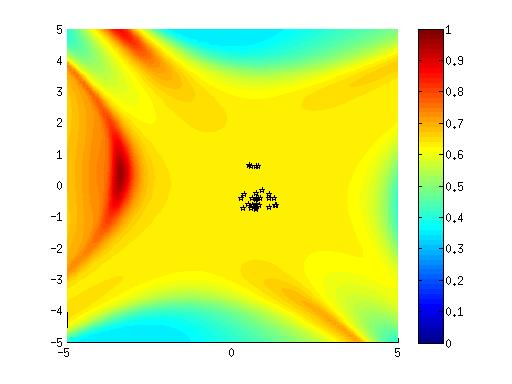
\includegraphics[width=\textwidth]{figures/GeneticAlgorithm/GPR7.jpg}
					\caption{\centerline{Tenth generation\\ Goldstein Price Function}}
					\label{GPR5}
				\end{subfigure}
				\quad
				\begin{subfigure}[b]{0.5\textwidth}
					\centering
					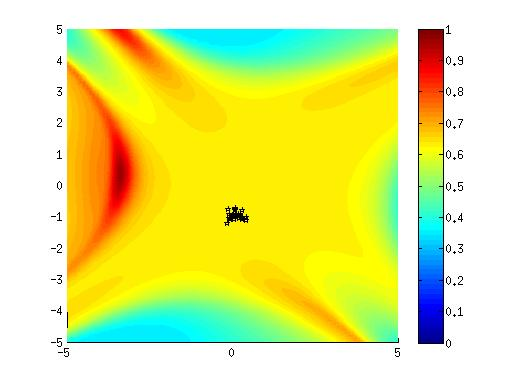
\includegraphics[width=\textwidth]{figures/GeneticAlgorithm/GPR9.jpg}
					\caption{\centerline{Final generation\\ Goldstein Price Function}}
					\label{GPR6}
				\end{subfigure}
				\caption{Convergence of populations over generations, Goldstein Price Function}
				\label{GPRT}
			\end{figure}

		\clearpage

		\subsection{Beale's function}

			Beale's function is defined by:
			\begin{equation}
				f(x,y) = (1.5-x+xy)^2+(2.25-x+xy^2)^2+(2.625-x+xy^3)^2
			\end{equation}
			The function has a minimum value of 0 at $(3,0.5)$.

			\begin{figure}[hb!]
				\centering
				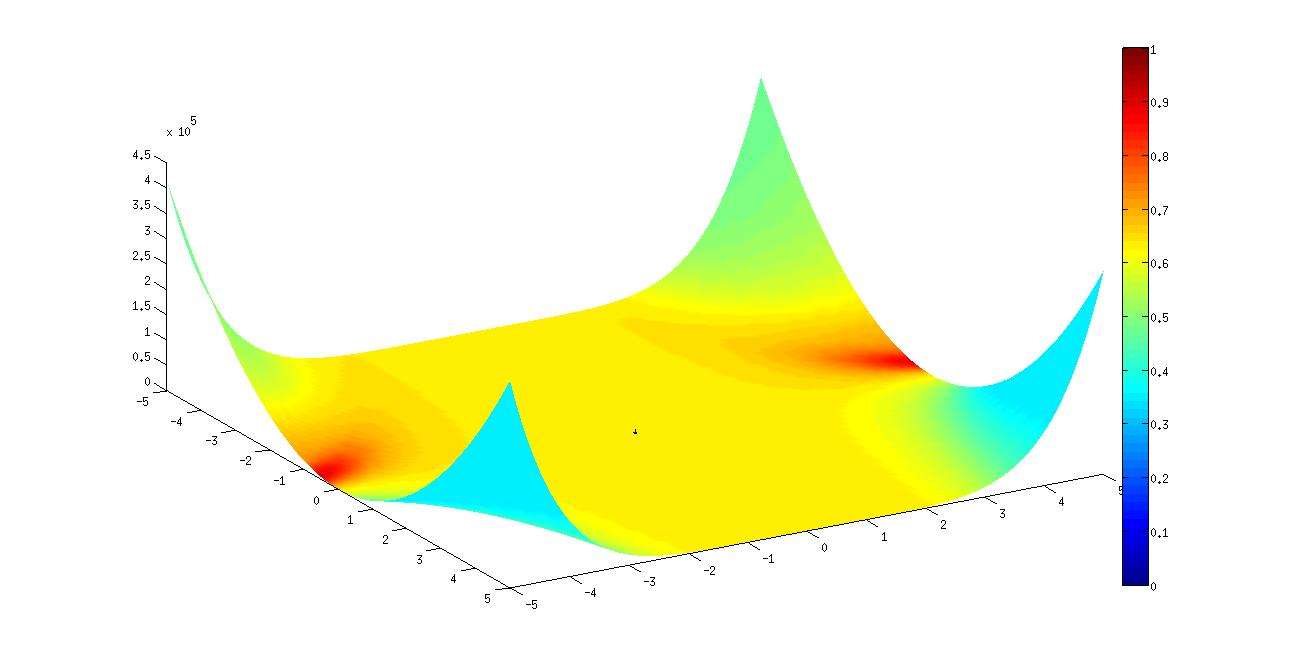
\includegraphics[width=\textwidth]{figures/GeneticAlgorithm/Beale.jpg}
				\caption{Beale's function}
				\label{B1}
			\end{figure}

			\begin{figure}[hb!]
				\centering
				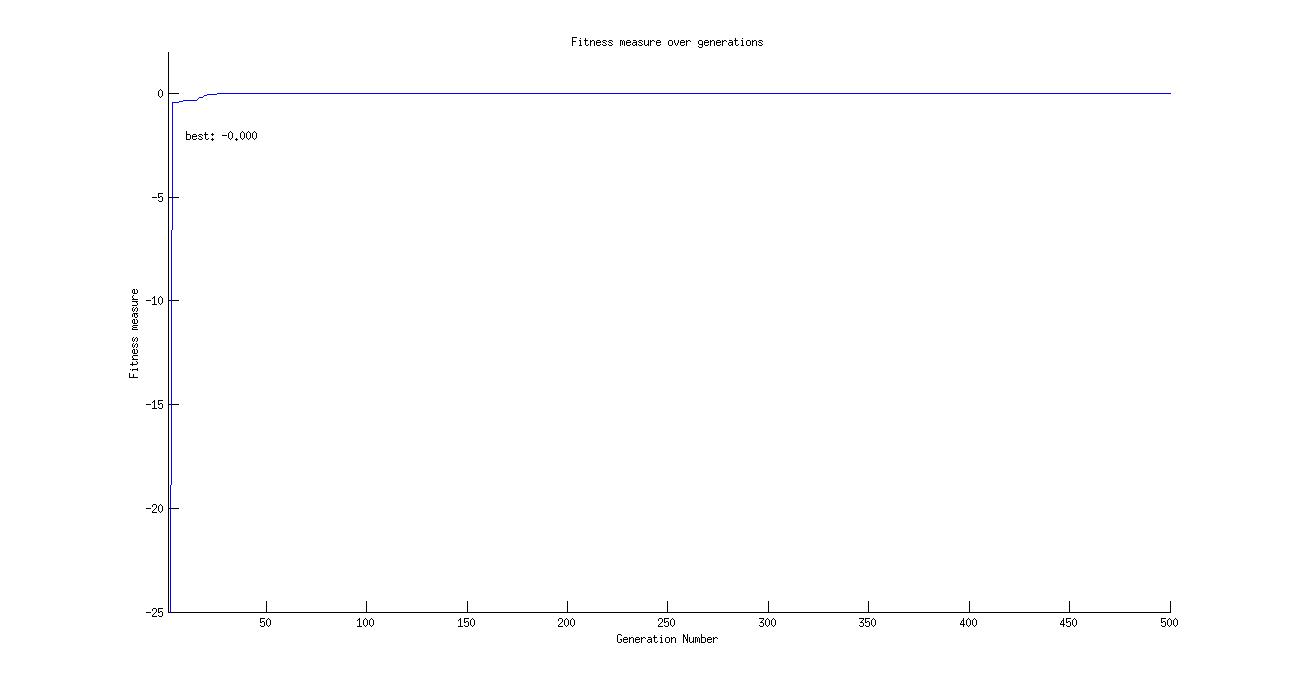
\includegraphics[width=\textwidth]{figures/GeneticAlgorithm/Beale_fitness_vs_generation.jpg}
				\caption{Progress of population best fitness over generations, Beale's function}
				\label{B1F}
			\end{figure}

			\begin{figure}
				\begin{subfigure}[b]{0.5\textwidth}
					\centering
					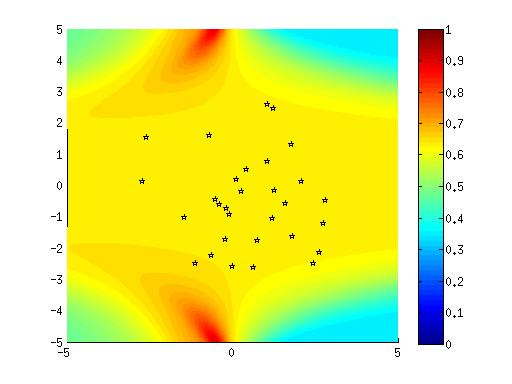
\includegraphics[width=\textwidth]{figures/GeneticAlgorithm/Beale1.jpg}
					\caption{\centerline{First generation\\ Beale's Function}}
					\label{B11}
				\end{subfigure}
				\quad
				\begin{subfigure}[b]{0.5\textwidth}
					\centering
					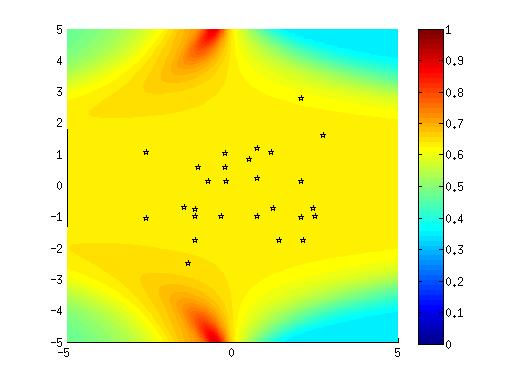
\includegraphics[width=\textwidth]{figures/GeneticAlgorithm/Beale2.jpg}
					\caption{\centerline{Third generation\\ Beale's Function}}
					\label{B12}
				\end{subfigure}

				\begin{subfigure}[b]{0.5\textwidth}
					\centering
					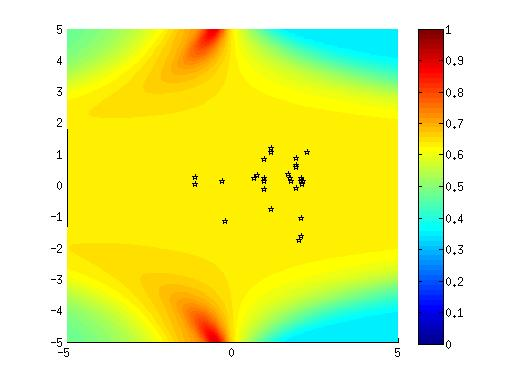
\includegraphics[width=\textwidth]{figures/GeneticAlgorithm/Beale4.jpg}
					\caption{\centerline{Fifth generation\\ Beale's Function}}
					\label{B13}
				\end{subfigure}
				\quad
				\begin{subfigure}[b]{0.5\textwidth}
					\centering
					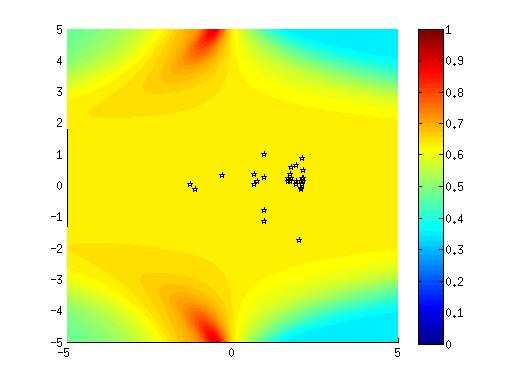
\includegraphics[width=\textwidth]{figures/GeneticAlgorithm/Beale5.jpg}
					\caption{\centerline{Ninth generation\\ Beale's Function}}
					\label{B14}
				\end{subfigure}

				\begin{subfigure}[b]{0.5\textwidth}
					\centering
					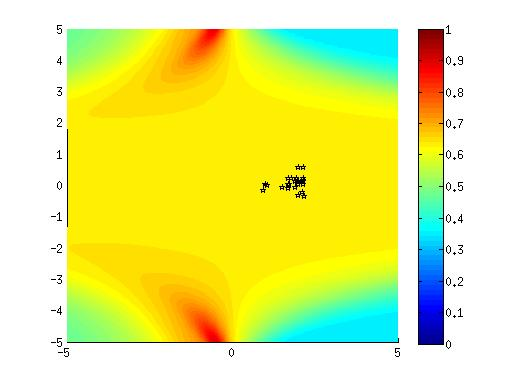
\includegraphics[width=\textwidth]{figures/GeneticAlgorithm/Beale7.jpg}
					\caption{\centerline{Tenth generation\\ Beale's Function}}
					\label{B15}
				\end{subfigure}
				\quad
				\begin{subfigure}[b]{0.5\textwidth}
					\centering
					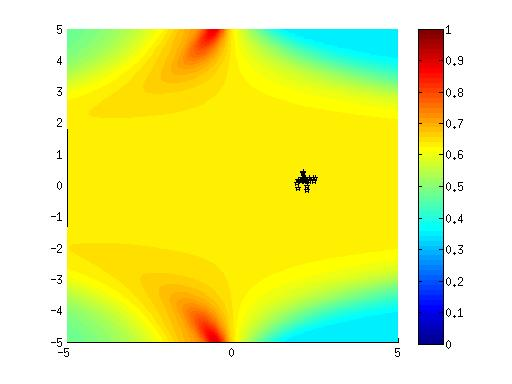
\includegraphics[width=\textwidth]{figures/GeneticAlgorithm/Beale9.jpg}
					\caption{\centerline{Final generation\\ Beale's Function}}
					\label{B16}
				\end{subfigure}
				\caption{Convergence of populations over generations, Beale's function}
				\label{Beale}
			\end{figure}

		\clearpage

		\subsection{Booth's function}

		Booth's function is defined as:
		\begin{equation}
			f(x,y)=(x+2y-7)^2+(2x+y-5)^2
		\end{equation}
		The function has a minima of 0 at $(1,3)$.

		\begin{figure}[hb!]
			\begin{subfigure}[b]{0.5\textwidth}
				\centering
				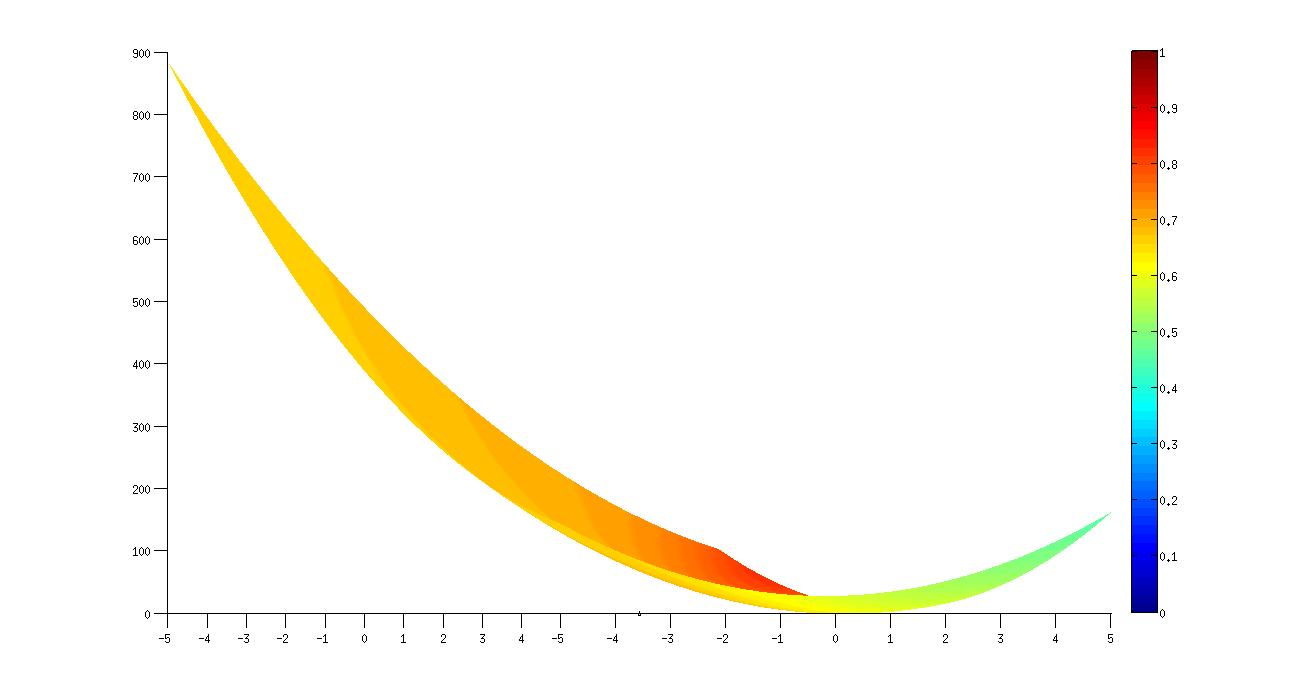
\includegraphics[width=1.2\textwidth]{figures/GeneticAlgorithm/BoothA.jpg}
				\caption{Booth's Function (A)}
				\label{B2A}
			\end{subfigure}
			\quad
			\begin{subfigure}[b]{0.5\textwidth}
				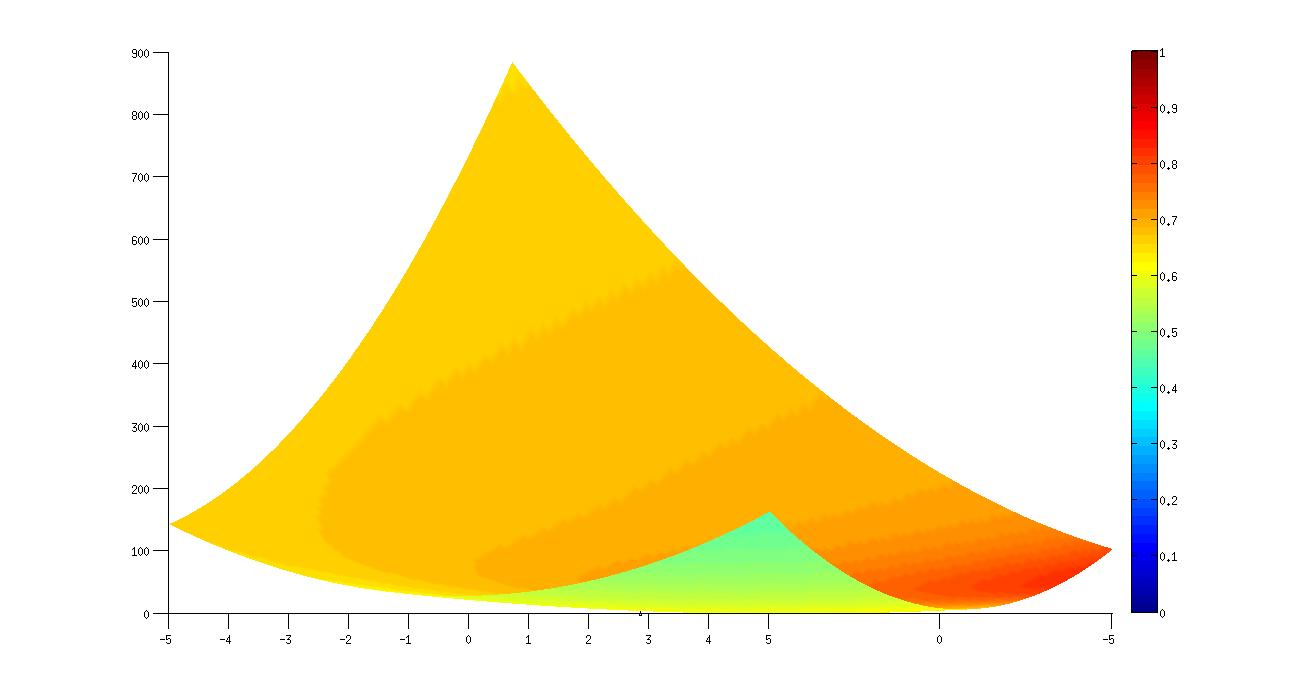
\includegraphics[width=1.2\textwidth]{figures/GeneticAlgorithm/BoothB.jpg}
				\caption{Booth's Function (B)}
				\label{B2B}
			\end{subfigure}
			\caption{Booth's function}
			\label{B2}
		\end{figure}

		\begin{figure}[hb!]
			\centering
			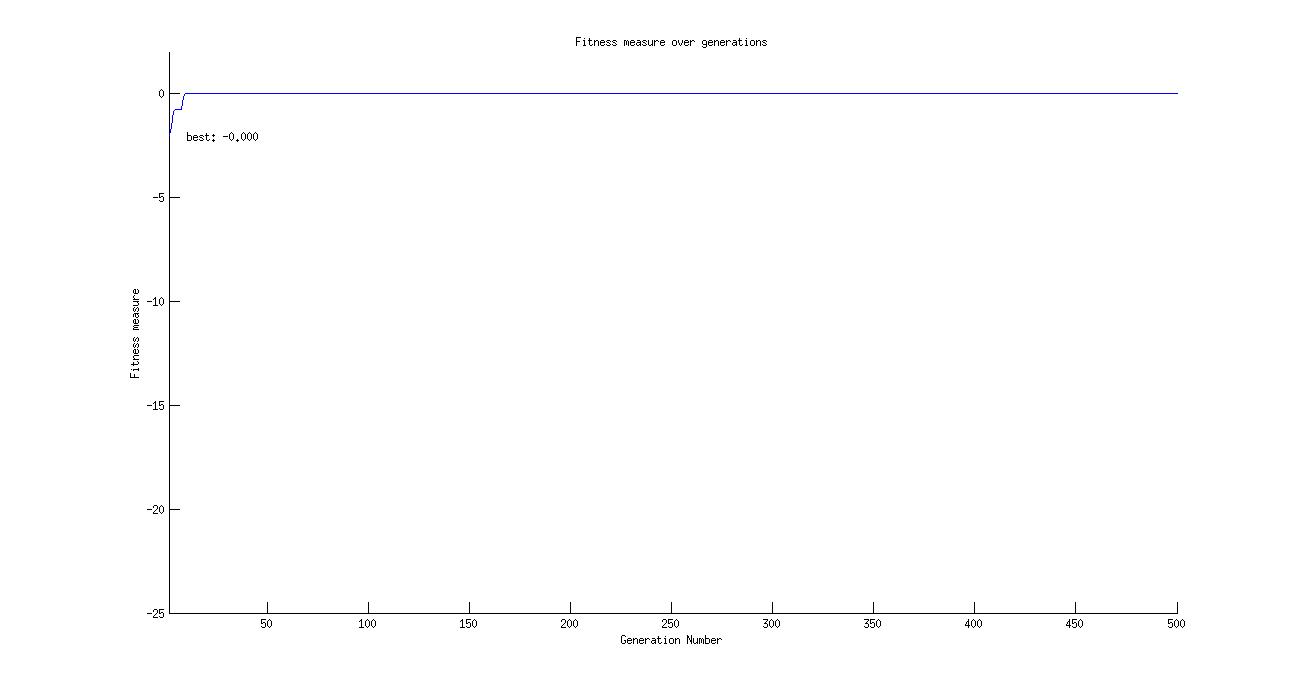
\includegraphics[width=\textwidth]{figures/GeneticAlgorithm/Booth_fitness_vs_generation.jpg}
			\caption{Progress of population best fitness over generations, Booth's function}
			\label{B2F}
		\end{figure}

		\begin{figure}
			\begin{subfigure}[b]{0.5\textwidth}
				\centering
				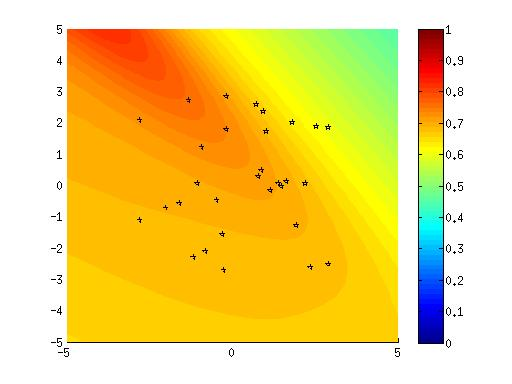
\includegraphics[width=\textwidth]{figures/GeneticAlgorithm/Booth1.jpg}
				\caption{\centerline{First generation\\ Booth's Function}}
				\label{B21}
			\end{subfigure}
			\quad
			\begin{subfigure}[b]{0.5\textwidth}
				\centering
				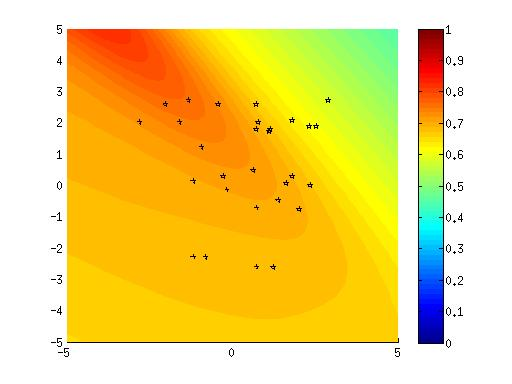
\includegraphics[width=\textwidth]{figures/GeneticAlgorithm/Booth2.jpg}
				\caption{\centerline{Third generation\\ Booth's Function}}
				\label{B22}
			\end{subfigure}

			\begin{subfigure}[b]{0.5\textwidth}
				\centering
				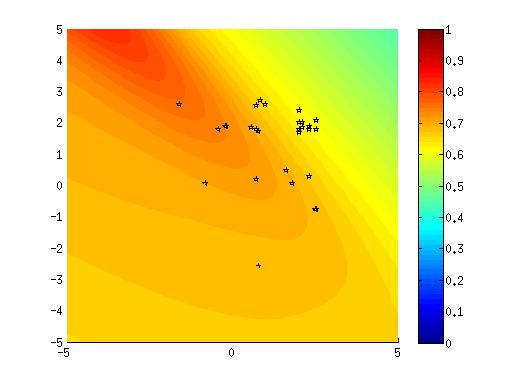
\includegraphics[width=\textwidth]{figures/GeneticAlgorithm/Booth4.jpg}
				\caption{\centerline{Fifth generation\\ Booth's Function}}
				\label{B23}
			\end{subfigure}
			\quad
			\begin{subfigure}[b]{0.5\textwidth}
				\centering
				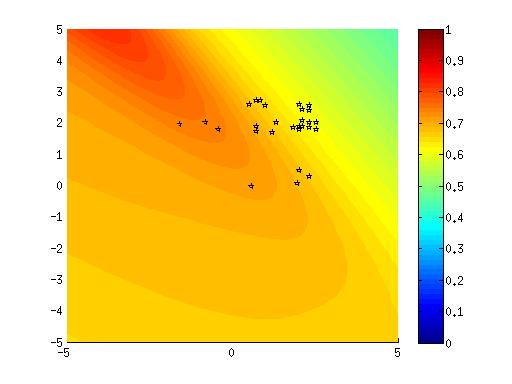
\includegraphics[width=\textwidth]{figures/GeneticAlgorithm/Booth5.jpg}
				\caption{\centerline{Ninth generation\\ Booth's Function}}
				\label{B24}
			\end{subfigure}

			\begin{subfigure}[b]{0.5\textwidth}
				\centering
				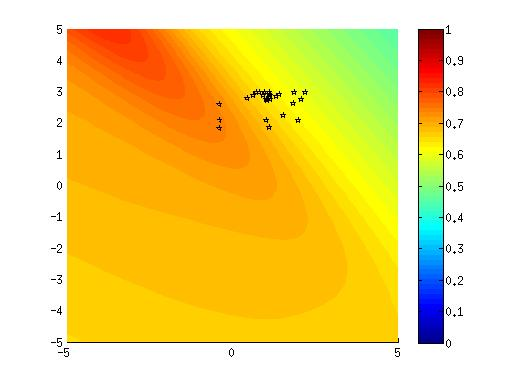
\includegraphics[width=\textwidth]{figures/GeneticAlgorithm/Booth7.jpg}
				\caption{\centerline{Tenth generation\\ Booth's Function}}
				\label{B25}
			\end{subfigure}
			\quad
			\begin{subfigure}[b]{0.5\textwidth}
				\centering
				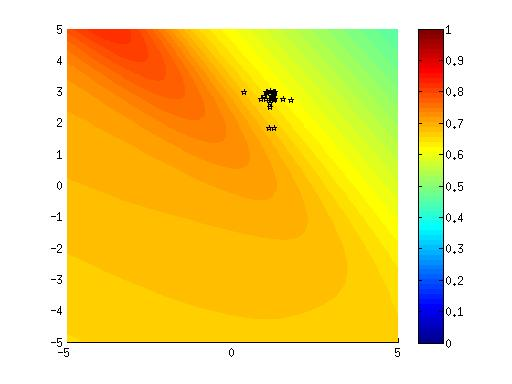
\includegraphics[width=\textwidth]{figures/GeneticAlgorithm/Booth9.jpg}
				\caption{\centerline{Final generation\\ Booth's Function}}
				\label{B26}
			\end{subfigure}
			\caption{Convergence of populations over generations, Booth's function}
			\label{Booth}
		\end{figure}

	\clearpage
\end{document}
